% Suggested text changes for the tower top DEL (chapter 04_WindTurbineControl_02_notBold.tex).
% Each block: the original lines (commented, "% OLD:") followed by the suggested new lines.
% The tables are in figures/figIPCThesis/tab_IPC_summary.tex and tab_AALC_summary.tex.

% ---- original line 706 (after: "\subsubsection*{Load Criteria: Blade $C_{\text{DEL},b} = J$ and tower ")
% OLD: Reducing the blade DEL is the main incentive for using IPC to decrease the Power Spectral Density (PSD) at 1P. A reduction at the 1P frequency does not influence the tower DEL, however, finding a controller that decreases the peak at 1P tends to also result in a lower PSD for a wider frequency range including the peak at 2P. Thus, a small decrease in the tower DEL is also achieved although this criterion is not included in the objective function. In Section~\ref{sec:CombinedIPC-TrailingEdgeFlapControl} it will be discussed that decreasing the PSD at the 2P frequency via the flaps does decrease the tower DELs further. 
Reducing the blade DEL is the main incentive for using IPC to decrease the Power Spectral Density (PSD) at 1P. A reduction at the 1P frequency does not influence the tower DEL, however, finding a controller that decreases the peak at 1P tends to also result in a lower PSD for a wider frequency range including the peak at 2P. Thus, a small decrease in the tower DEL is also achieved although this criterion is not included in the objective function. In Section~\ref{sec:CombinedIPC-TrailingEdgeFlapControl} it will be discussed that decreasing the PSD at the 2P frequency via the flaps does decrease the tower DELs further. In addition to the tower base DEL $C_{\text{DEL},t,\text{Base}}$, the DEL of the tower top fore-aft bending moment $C_{\text{DEL},t,\text{Top}}$ is evaluated, which is affected directly by the rotor tilt moment. Both tower DELs are calculated with the Wöhler exponent of steel. 

% ---- original line 815 (after: "")
% OLD: Above rated, the blade DEL decreases by 19\% to 22\%, and from 18\,m/s on by 23\% to 24\%, for all three datasets. The reduction grows with the wind speed: for the second verification set of turbulence class~B, it increases from 12\% to 15\% between 12 and 16\,m/s to 24\% to 27\% from 20\,m/s on. The gains optimized at a single wind speed hence carry over to the whole of Region~III and to both verification sets, so that no gain scheduling is required above rated. The tower base DEL is not changed considerably, with criteria between 0.99 and 1.01; the largest increase of a single wind speed is 3\% at 18\,m/s for turbulence class~B. Close to rated wind speed, the mean power decreases by up to 0.6\% and its standard deviation increases slightly, so that the power criteria above rated are 1.00 and 1.01 to 1.02. The pitch rate reaches the limit of 8\textdegree/s at all wind speeds, and the actuator power is increased by a factor of 5.4 to 5.7 above rated and of 5.8 to 6.0 from 18\,m/s on. Compared with the AALC (Table~\ref{tabone}), the IPC achieves about the same blade DEL reduction above rated (AALC: 19\% to 23\%), but at a clearly higher actuator power (AALC: factor 3.9 to 4.0); from 18\,m/s on, the AALC reduces the blade DEL slightly more (22\% to 26\%).
Above rated, the blade DEL decreases by 19\% to 22\%, and from 18\,m/s on by 23\% to 24\%, for all three datasets. The reduction grows with the wind speed: for the second verification set of turbulence class~B, it increases from 12\% to 15\% between 12 and 16\,m/s to 24\% to 27\% from 20\,m/s on. The gains optimized at a single wind speed hence carry over to the whole of Region~III and to both verification sets, so that no gain scheduling is required above rated. The tower base DEL is not changed considerably, with criteria between 0.99 and 1.01; the largest increase of a single wind speed is 3\% at 18\,m/s for turbulence class~B. The tower top DEL is reduced slightly, by 2\% to 4\% above rated and by 3\% to 6\% at 18\,m/s. Close to rated wind speed, the mean power decreases by up to 0.6\% and its standard deviation increases slightly, so that the power criteria above rated are 1.00 and 1.01 to 1.02. The pitch rate reaches the limit of 8\textdegree/s at all wind speeds, and the actuator power is increased by a factor of 5.4 to 5.7 above rated and of 5.8 to 6.0 from 18\,m/s on. Compared with the AALC (Table~\ref{tabone}), the IPC achieves about the same blade DEL reduction above rated (AALC: 19\% to 23\%), but at a clearly higher actuator power (AALC: factor 3.9 to 4.0); from 18\,m/s on, the AALC reduces the blade DEL slightly more (22\% to 26\%).

% ---- original line 968 (after: "Apart from the blade root flapwise moment, the influence of the obtain")
% OLD: Table~\ref{tabone} contains the five evaluation criteria to quantify the effect of the AALC: blade and tower base DEL, mean of generated power $\bar{P}_{g}$, its standard deviation $\sigma P$, and actuator power $C_{\text{Act}}$, Equation~\eqref{eq:CAct}, normalized by simulations without AALC for the same wind test cases. From 10\,m/s on, the parameters optimized at 18\,m/s are used. Below, the AALC parameters are scheduled with the parameters optimized separately at 4, 6, and 8\,m/s. The criteria are averaged over five wind speed ranges: all wind speeds, the wind speeds below and above rated, the wind speeds from 18\,m/s, and the optimization wind speed of 18\,m/s.
Table~\ref{tabone} contains the evaluation criteria to quantify the effect of the AALC: blade, tower base, and tower top DEL, mean of generated power $\bar{P}_{g}$, its standard deviation $\sigma P$, and actuator power $C_{\text{Act}}$, Equation~\eqref{eq:CAct}, normalized by simulations without AALC for the same wind test cases. From 10\,m/s on, the parameters optimized at 18\,m/s are used. Below, the AALC parameters are scheduled with the parameters optimized separately at 4, 6, and 8\,m/s. The criteria are averaged over five wind speed ranges: all wind speeds, the wind speeds below and above rated, the wind speeds from 18\,m/s, and the optimization wind speed of 18\,m/s.

% ---- original line 1000 (after: "")
% OLD: Above rated, the blade DEL decreases by 19\% to 23\%, and from 18\,m/s on by 22\% to 26\%, with the largest reduction for the second verification set of turbulence class~B. The parameters optimized at a single wind speed hence carry over to the whole of Region~III and to both verification sets, so that no gain scheduling is required above rated. The tower base DEL is not changed considerably above rated, with criteria between 0.99 and 1.00; the largest increase of a single wind speed is 3\% at 18\,m/s for turbulence class~B. Below rated, the blade DEL is reduced by 19\% for the optimization set and by 15\% for the second verification set, but only by 3\% for the first verification set, i.e., the parameters optimized below rated do not carry over reliably to other wind fields. Here, the tower base DEL is reduced by 4\% to 7\%. Including all wind speeds, the blade DEL is reduced by 14\% to 22\%.
Above rated, the blade DEL decreases by 19\% to 23\%, and from 18\,m/s on by 22\% to 26\%, with the largest reduction for the second verification set of turbulence class~B. The parameters optimized at a single wind speed hence carry over to the whole of Region~III and to both verification sets, so that no gain scheduling is required above rated. The tower base DEL is not changed considerably above rated, with criteria between 0.99 and 1.00; the largest increase of a single wind speed is 3\% at 18\,m/s for turbulence class~B. The tower top DEL, in contrast, is reduced by 5\% to 8\% above rated and by 5\% to 10\% at 18\,m/s, i.e., more than by the IPC alone (Table~\ref{tab:IPC_summary}: 2\% to 4\% above rated). Below rated, the blade DEL is reduced by 19\% for the optimization set and by 15\% for the second verification set, but only by 3\% for the first verification set, i.e., the parameters optimized below rated do not carry over reliably to other wind fields. Here, the tower base DEL is reduced by 4\% to 7\% and the tower top DEL by 3\% to 8\%. Including all wind speeds, the blade DEL is reduced by 14\% to 22\%.

% ---- original line 1033 (after: "PI baseline on the same plant and with the same pitch rate limit, so v")
% OLD: indicate an improvement. The blade and tower DELs are computed by rainflow counting with
% OLD: W\"ohler exponents of 10 for the blades, summed over the three blades, and 4 for the steel
% OLD: tower; all criteria are evaluated from 66\,s onwards to exclude the start-up. Mdl2 contains
indicate an improvement. The blade DEL and the DELs of the tower base and the tower top fore-aft moments are computed by
rainflow counting with W\"ohler exponents of 10 for the blades, summed over the three blades, and
4 for the steel tower; all criteria are evaluated from 66\,s onwards to exclude the start-up. Mdl2 contains

% ---- original line 1037 (after: "neither blade loads nor a pitch moment. For the qLMPC on Mdl2, the sta")
% OLD: tower top fore-aft acceleration replaces the tower DEL, no blade DEL is given, and $C_\text{Act}$
tower top fore-aft acceleration replaces the tower base DEL, no blade and tower top DELs are given, and $C_\text{Act}$

% ---- original line 1045 (after: "        \includegraphics[width=0.6\textwidth]{figures/figures_WESC25/a")
% OLD:         \caption[Evaluation criteria of qLMPC, IPC, and AALC for turbulent wind at a pitch rate limit of 8\textdegree/s]{Evaluation criteria of the controllers for turbulent wind (18\,m/s mean, IEC turbulence class~B, second verification set) and a pitch rate limit of 8\textdegree/s, normalized by the PI baseline with the same rate limit: blade and tower DELs $C_{\mathrm{DEL},b}$ and $C_{\mathrm{DEL},t}$, mean power $C_{\bar{P}}$, power standard deviation $C_{\delta P}$, and actuator power $C_\text{Act}$. (a)~qLMPC, (b)~IPC and AALC, (c)~qLMPC combined with IPC. $^*$qLMPC on Mdl2 (no model mismatch): $C_\text{Act}$ with the pitch moment estimated from a model fitted to FAST, $C_{\mathrm{DEL},t}$ replaced by the standard deviation of the tower top fore-aft acceleration, no blade DEL.}
        \caption[Evaluation criteria of qLMPC, IPC, and AALC for turbulent wind at a pitch rate limit of 8\textdegree/s]{Evaluation criteria of the controllers for turbulent wind (18\,m/s mean, IEC turbulence class~B, second verification set) and a pitch rate limit of 8\textdegree/s, normalized by the PI baseline with the same rate limit: blade, tower base, and tower top DELs $C_{\mathrm{DEL},b}$, $C_{\mathrm{DEL},t,\mathrm{Base}}$, and $C_{\mathrm{DEL},t,\mathrm{Top}}$, mean power $C_{\bar{P}}$, power standard deviation $C_{\delta P}$, and actuator power $C_\text{Act}$. (a)~qLMPC, (b)~IPC and AALC, (c)~qLMPC combined with IPC. $^*$qLMPC on Mdl2 (no model mismatch): $C_\text{Act}$ with the pitch moment estimated from a model fitted to FAST, $C_{\mathrm{DEL},t,\mathrm{Base}}$ replaced by the standard deviation of the tower top fore-aft acceleration, no blade and tower top DELs.}

% ---- original line 1060 (after: "wind fluctuations with fast pitch action. On FAST, the qLMPC with notc")
% OLD: power standard deviation by 33\%, but it does not reduce the blade DEL, increases the tower DEL
% OLD: by 33\%, and requires the highest actuator power of all controllers without IPC, 6.5 times that
power standard deviation by 33\%, but it does not reduce the blade DEL, increases the tower base DEL
by 33\% while the tower top DEL remains unchanged, and requires the highest actuator power of all controllers without IPC, 6.5 times that

% ---- original line 1067 (after: "Panel~(b) shows the IPC and the AALC, which act on the blade loads. Th")
% OLD: 21\% and 23\%, with a small increase of the tower DEL by 6\%, and leave the power standard
21\% and 23\% and the tower top DEL by 9\% and 13\%, with a small increase of the tower base DEL by 6\%, and leave the power standard

% ---- original line 1073 (after: "Panel~(c) shows the qLMPC designs combined with IPC. Adding IPC reduce")
% OLD: and 15\% instead of 2\%, while the tower DEL and the power standard deviation remain close to the
% OLD: values of the qLMPC alone. The additional individual pitch action increases the actuator power to
and 15\% instead of 2\%, while the tower base DEL and the power standard deviation remain close to the
values of the qLMPC alone. In contrast to the IPC on OpenFAST, the combination increases the tower top DEL by 8\%. The additional individual pitch action increases the actuator power to

% ==== Figures (line numbers on the current main) ====

% ---- original line 1047 (after: "")
% Bar plot (fig:EvalCrit1) and Pareto plot (fig:CtrlCompAll) side by side in one figure;
% it replaces this figure and the Pareto figure at line 1082 (next block).
% The old labels are kept for the subfigures, so \ref{fig:EvalCrit1} and
% \ref{fig:CtrlCompAll} in the text still work (they then print e.g. 4.12a and 4.12b);
% fig:CtrlCompBarPareto refers to the whole figure.
% The panels inside the plots have no letters (a), (b), (c) any more; the caption
% and the text (blocks below) call them top, middle, and bottom panel.
% OLD: \begin{figure}[htbp]
% OLD:     \begin{center}
% OLD:         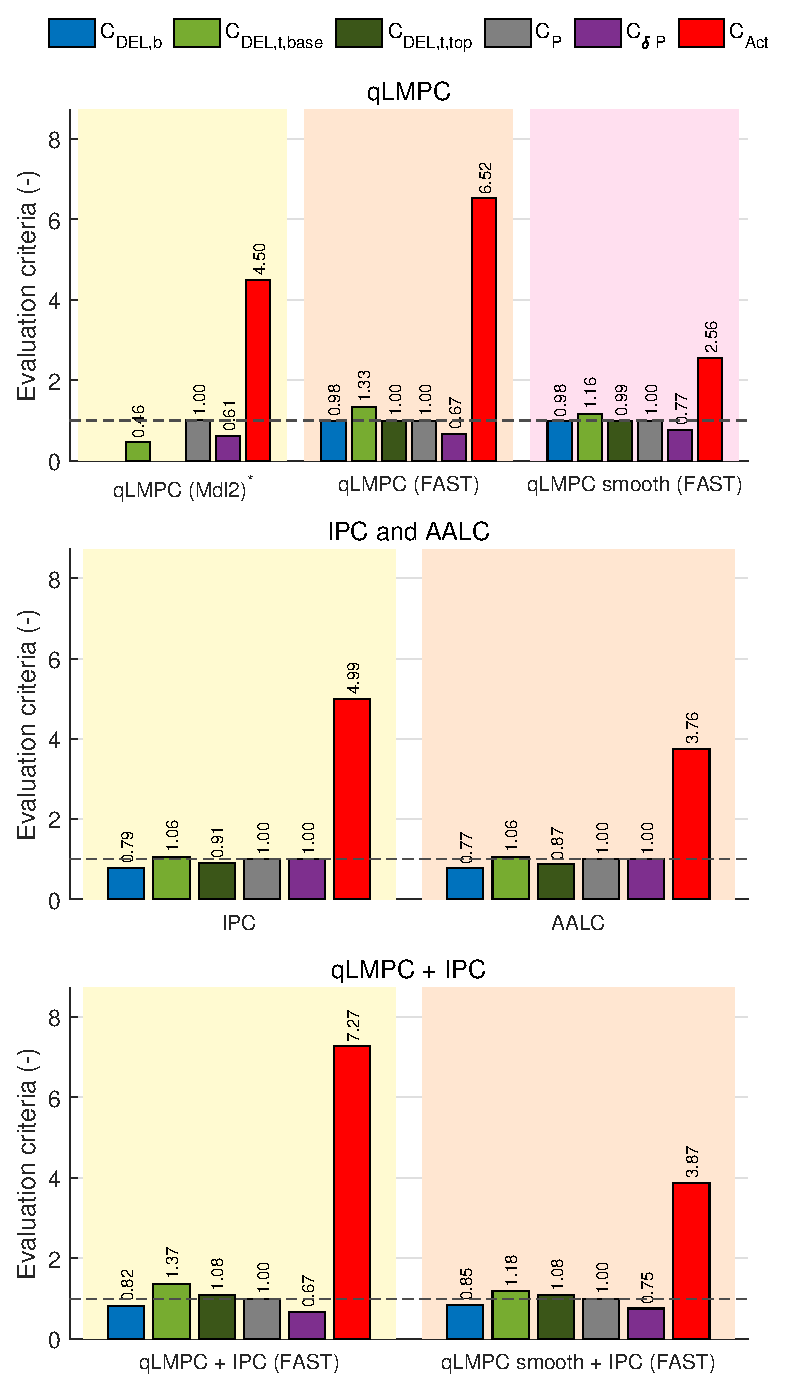
\includegraphics[width=0.6\textwidth]{figures/figures_WESC25/afig01_IPCMPCbar.eps}
% OLD:         \caption[Evaluation criteria of qLMPC, IPC, and AALC for turbulent wind at a pitch rate limit of 8\textdegree/s]{Evaluation criteria of the controllers for turbulent wind (18\,m/s mean, IEC turbulence class~B, second verification set) and a pitch rate limit of 8\textdegree/s, normalized by the PI baseline with the same rate limit: blade and tower DELs $C_{\mathrm{DEL},b}$ and $C_{\mathrm{DEL},t}$, mean power $C_{\bar{P}}$, power standard deviation $C_{\delta P}$, and actuator power $C_\text{Act}$. (a)~qLMPC, (b)~IPC and AALC, (c)~qLMPC combined with IPC. $^*$qLMPC on Mdl2 (no model mismatch): $C_\text{Act}$ with the pitch moment estimated from a model fitted to FAST, $C_{\mathrm{DEL},t}$ replaced by the standard deviation of the tower top fore-aft acceleration, no blade DEL.}
% OLD:         \label{fig:EvalCrit1}
% OLD:     \end{center}
% OLD: \end{figure}
\begin{figure}[htbp]
    \centering
    \subfloat[Bar plot\label{fig:EvalCrit1}]{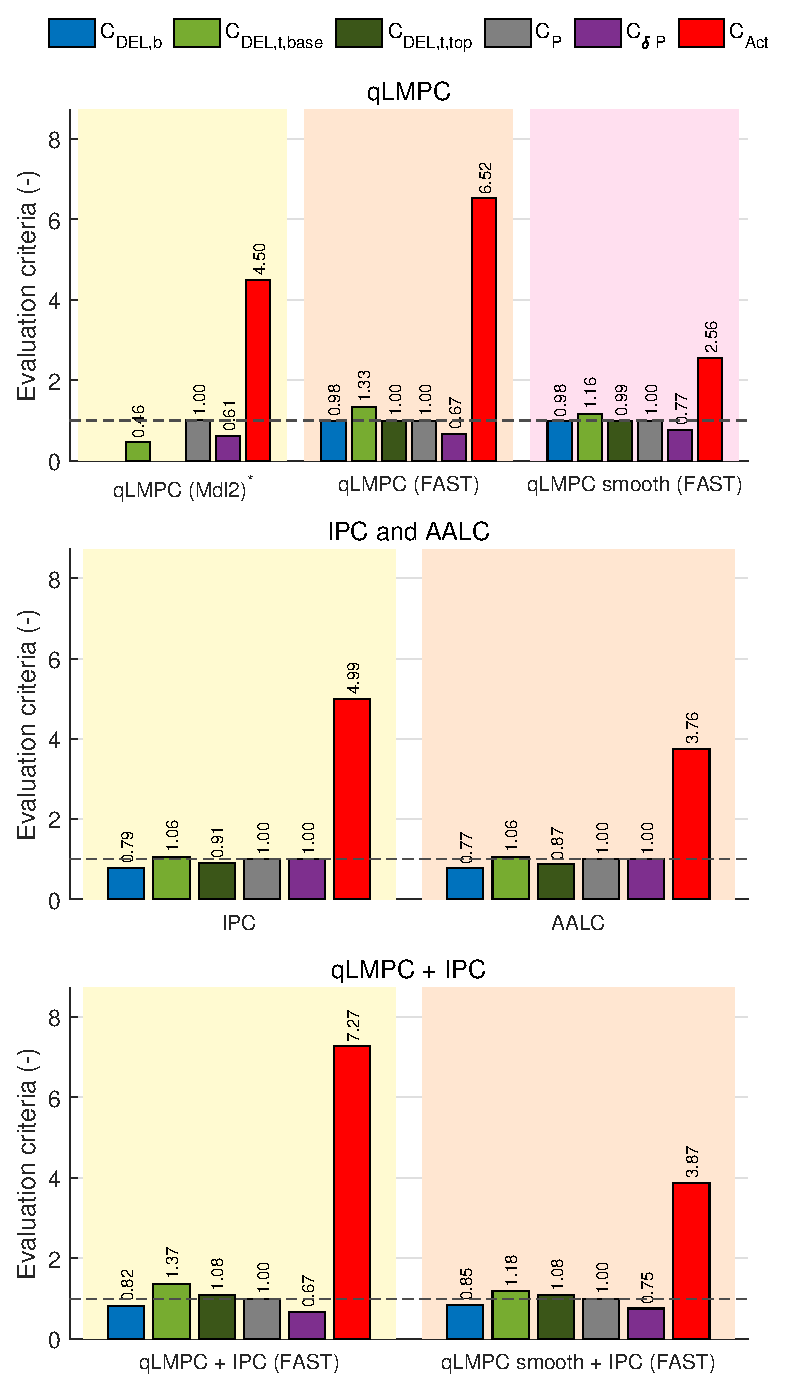
\includegraphics[width=0.49\textwidth]{figures/figures_WESC25/afig01_IPCMPCbar.eps}}\hfill
    \subfloat[Pareto plot\label{fig:CtrlCompAll}]{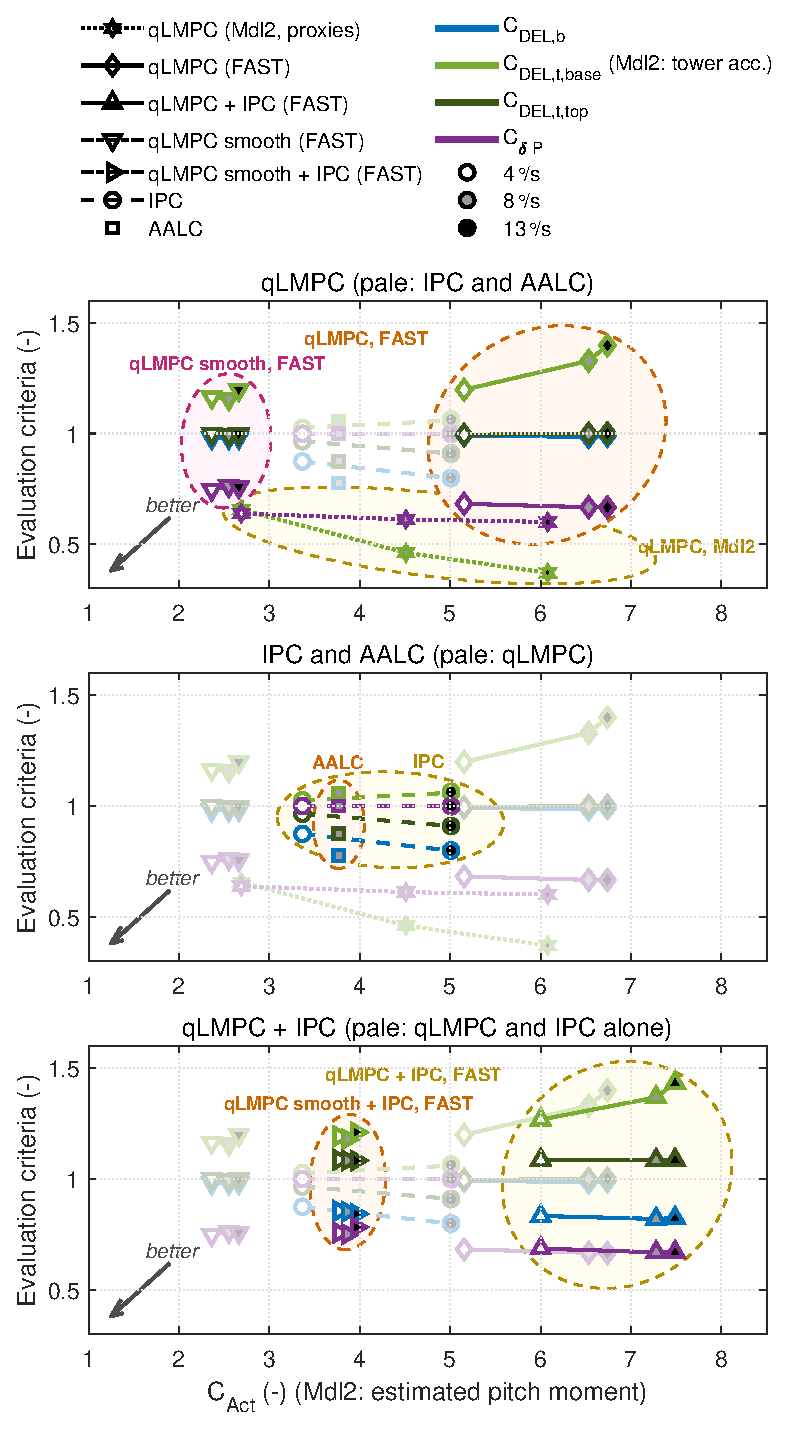
\includegraphics[width=0.49\textwidth]{figures/figures_WESC25/afig01_IPCMPCpareto.eps}}
    \caption[Evaluation criteria of qLMPC, IPC, and AALC for turbulent wind]{Evaluation criteria of the controllers for turbulent wind (18\,m/s mean, IEC turbulence class~B, second verification set), normalized by the PI baseline with the same pitch rate limit. Panels: qLMPC (top), IPC and AALC (middle), qLMPC combined with IPC (bottom). (a)~Bar plot at a pitch rate limit of 8\textdegree/s: blade DEL $C_{\mathrm{DEL},b}$, tower base and tower top DELs $C_{\mathrm{DEL},t,\mathrm{Base}}$ and $C_{\mathrm{DEL},t,\mathrm{Top}}$, mean power $C_{\bar{P}}$, power standard deviation $C_{\delta P}$, and actuator power $C_\text{Act}$. (b)~Pareto plot: $C_{\mathrm{DEL},b}$ (blue), $C_{\mathrm{DEL},t,\mathrm{Base}}$ (green), $C_{\mathrm{DEL},t,\mathrm{Top}}$ (dark green), and $C_{\delta P}$ (purple) over $C_\text{Act}$ for the pitch rate limits 4\textdegree/s (white markers), 8\textdegree/s (grey), and 13\textdegree/s (black); the controllers of the other panels are shown pale. The dashed ovals enclose all points of one controller; their colour matches the background of the same controller in the same panel of the bar plot. $^*$qLMPC on Mdl2 (no model mismatch): tower top fore-aft acceleration instead of the tower base DEL, no blade and tower top DELs, $C_\text{Act}$ with the pitch moment estimated from a model fitted to FAST. The arrow points towards better results.}
    \label{fig:CtrlCompBarPareto}
\end{figure}

% ---- original line 1082 (after: "")
% Pareto figure: delete, it is now part of the figure above (no new lines).
% OLD: \begin{figure}[htbp]
% OLD:     \begin{center}
% OLD:         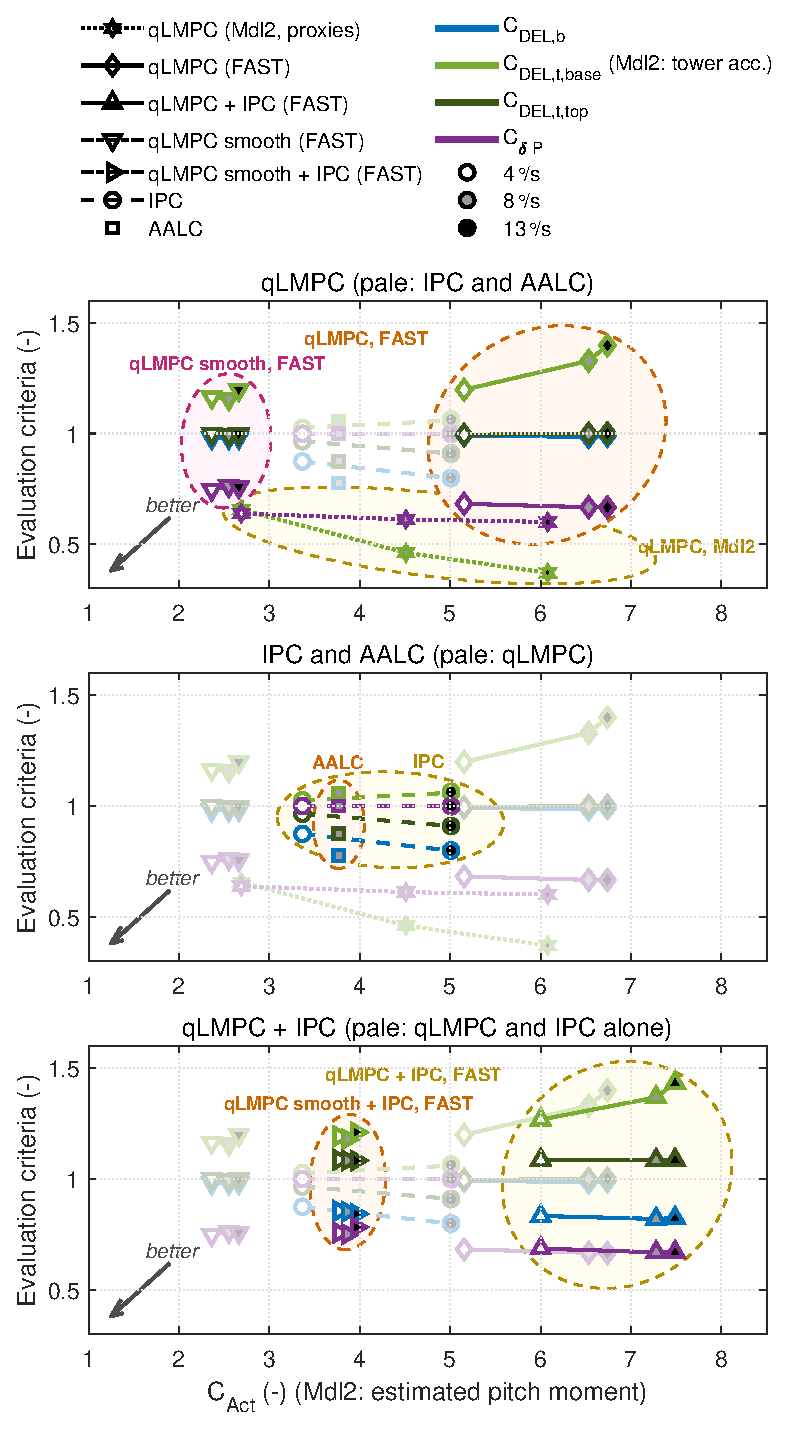
\includegraphics[width=0.6\textwidth]{figures/figures_WESC25/afig01_IPCMPCpareto.eps}
% OLD:         \caption[Evaluation criteria of qLMPC, IPC, and AALC over the actuator power for turbulent wind]{Evaluation criteria $C_{\mathrm{DEL},b}$ (blue), $C_{\mathrm{DEL},t}$ (green), and $C_{\delta P}$ (purple) over the actuator power $C_\text{Act}$ for turbulent wind (18\,m/s mean, IEC turbulence class~B, second verification set), normalized by the PI baseline with the same pitch rate limit. Marker fill: pitch rate limit 4\textdegree/s (white), 8\textdegree/s (grey), and 13\textdegree/s (black). (a)~qLMPC on Mdl2 and FAST, IPC and AALC pale, (b)~IPC and AALC, qLMPC pale, (c)~qLMPC combined with IPC on FAST, qLMPC and IPC alone pale. qLMPC on Mdl2: tower top fore-aft acceleration instead of the tower DEL, $C_\text{Act}$ with the estimated pitch moment. The arrow points towards better results.}
% OLD:         \label{fig:CtrlCompAll}
% OLD:     \end{center}
% OLD: \end{figure}

% ==== Panel references: top, middle, bottom instead of (a), (b), (c) ====

% ---- original line 1059 (after: "")
% OLD: Panel~(a) shows the qLMPC. On Mdl2, i.e.\ without model mismatch, the qLMPC reduces the power
The top panel shows the qLMPC. On Mdl2, i.e.\ without model mismatch, the qLMPC reduces the power

% ---- original line 1071 (after: "")
% OLD: Panel~(b) shows the IPC and the AALC, which act on the blade loads. They reduce the blade DEL by
The middle panel shows the IPC and the AALC, which act on the blade loads. They reduce the blade DEL by

% ---- original line 1077 (after: "")
% OLD: Panel~(c) shows the qLMPC designs combined with IPC. Adding IPC reduces the blade DEL by 18\%
The bottom panel shows the qLMPC designs combined with IPC. Adding IPC reduces the blade DEL by 18\%

% ---- original line 1098 (after: "")
% OLD: Panel~(a) highlights the qLMPC. On Mdl2, higher pitch rate limits continuously reduce the tower
The top panel highlights the qLMPC. On Mdl2, higher pitch rate limits continuously reduce the tower

% ---- original line 1110 (after: "")
% OLD: Panel~(b) highlights the IPC and the AALC. The IPC reduces the blade DEL from 0.87 at
The middle panel highlights the IPC and the AALC. The IPC reduces the blade DEL from 0.87 at

% ---- original line 1117 (after: "")
% OLD: Panel~(c) highlights the combination of qLMPC and IPC. Compared with the pale qLMPC curves, adding
The bottom panel highlights the combination of qLMPC and IPC. Compared with the pale qLMPC curves, adding

% ==== qLMPC on FAST: new subsection and references to it (line numbers on main c5be1a2) ====

% ---- original line 517 (after: "%; only the projection factor $\cos(5^\circ)$ remains in the plant of ")
% New subsection before \subsection{Results} (line 518): insert, no OLD lines.
% It describes only the two FAST designs of the comparison (qlmpcDesign.m: flapNotch and
% flapNotchSmooth12, qLMPC repository); table values from experiments/results_summary.md
% (FAST 18 m/s tuning wind, 60-600 s).
% CHECK: the IPC gain set that is scaled by 0.3 (ipc_dlr gain set 2 of initDLRparameter).
\subsection{Adaptations for the Application to FAST}\label{sec:qLMPCFAST}

The qLMPC design described above is tuned on the qLPV model Mdl2, which also serves as its prediction model. Applied to the FAST model of the NREL 5-MW turbine in turbulent wind, this design does not work: its fast pitch action excites structural modes of FAST that are not contained in the prediction model, i.e.\ the tower fore-aft mode at about 0.32\,Hz, the blade passing frequency 3P, and the drivetrain mode at 1.64\,Hz. For FAST, two designs are therefore derived, the notch filter design and the smooth design, which are evaluated in Section~\ref{subsec:ComparisonWindTurbineControlDesigns}. They differ from the design above as described in the following; the optimization algorithm of Section~\ref{sec:qLMPCOptimizationAlgo} remains unchanged.

\textbf{Prediction model and weights.} The prediction model is extended by the tower fore-aft and the blade flap dynamics of Mdl2. The tower states are estimated from the measured tower top fore-aft acceleration by leaky integration with a corner frequency of 0.02\,Hz. The blade flap state is not measured; it is obtained by integrating the blade equation of Mdl2, driven by the measured tower motion and the deviations of rotor speed, pitch angle, and wind speed from their slow means, which is stable due to the aerodynamic damping of the blades. Instead of the pitch reference $r_\beta$, the rotor speed is tracked: the weight on the pitch angle is zero, the rotor speed and the rotor and generator speed increments are weighted with 1000, the pitch increments with $10^5$, and the terminal weight is $10\,\bm{Q}_{\text{WT}}$ instead of $1000\,\bm{Q}_{\text{WT}}$. The controller sample time is 0.04\,s, which extends the prediction horizon from 0.32\,s to 1.6\,s with the same number of prediction steps. The controller is scheduled with the hub height wind speed filtered with the rotor-effective wind filter $V_{\text{filt},\tau}$ introduced at the end of Chapter~\ref{sec:WindTurbineqLPVModels}.

\textbf{Notch filters.} The measured rotor and generator speeds are filtered with notch filters
\begin{align*}
    N(s) = \frac{s^2 + 2\zeta_z\omega_0 s + \omega_0^2}{s^2 + 2\zeta_p\omega_0 s + \omega_0^2},
\end{align*}
with $\omega_0 = 2\pi f_0$ at $f_0 = 0.605$\,Hz (3P at the rated rotor speed of 12.1\,rpm) and $f_0 = 1.64$\,Hz (drivetrain mode of FAST), the pole damping $\zeta_p = 0.1$ and the zero damping $\zeta_z = 0.01$, discretized with the Tustin method with prewarping. They prevent the controller from reacting to the rotor speed oscillations at these frequencies. This design is referred to as the notch filter design.

\textbf{Smooth design.} With a sample time of 0.04\,s, the step-wise changes of the pitch reference still cause pitch activity between 2.4\,Hz and 6\,Hz. For the smooth design, the controller sample time of the notch filter design is increased to 0.12\,s, which extends the horizon to 4.8\,s, and the pitch reference is ramped linearly from the current value to the new reference at the plant sample time of 8\,ms instead of changing step-wise.

\begin{table}[htbp]
    \centering
    \caption[qLMPC designs for the application to FAST]{qLMPC designs for the application to FAST: standard deviations of rotor speed, power, tower top fore-aft acceleration, and pitch rate on FAST for the turbulent 18\,m/s wind used for the tuning, evaluated from 60\,s to 600\,s.}
    \label{tab:qLMPCFAST}
    \begin{tabular}{l c rrrr}
        \toprule
        Design & Sample time & Rotor speed & Power & Tower acc. & Pitch rate \\
        & (s) & (rpm) & (kW) & (m/s$^2$) & (\textdegree/s) \\
        \midrule
        PI baseline & -- & 0.286 & 120 & 0.190 & 0.62 \\
        Notch filter design & 0.04 & 0.086 & 38 & 0.290 & 3.60 \\
        Smooth design & 0.12 & 0.155 & 66 & 0.233 & 1.65 \\
        \bottomrule
    \end{tabular}
\end{table}

Both designs reduce the standard deviations of rotor speed and power considerably compared with the PI baseline, by about 70\% for the notch filter design and 45\% for the smooth design, see Table~\ref{tab:qLMPCFAST}. The smooth design requires less than half of the pitch activity of the notch filter design. Neither design reaches the tower fore-aft acceleration of the PI baseline, which is 53\% and 23\% higher. For the combination with individual pitch control, the IPC of Section~\ref{section:Individal Pitch PI Control} is added to the collective pitch command of the qLMPC, and the qLMPC receives the mean blade pitch angle as feedback. The IPC gains are not optimized for the combination. On FAST, the unscaled gains increase the blade root moments and the tower acceleration instead of reducing them. They were therefore scaled by hand on the notch filter design with the factors 0.1, 0.3, and 0.5, and the factor 0.3, which gave the lowest blade root moments, is used without the tower damping term for both designs and all pitch rate limits, i.e.\ without retuning for the smooth design.

% ---- original line 519 (after: "\subsection{Results} \label{quasiLPVMPCResults}")
% Sentence appended at the end of the paragraph.
% OLD: The velocity-based qLMPC is evaluated in two scenarios, similar to those used for model verification in Section~\ref{subsec:ResultsqLPVModel}. As in \cite{dittmer2021velocity}, the qLPV model Mdl2 is used as the plant. The controller model consists of a subset of its states with identical parameters, chosen to remain close to the model in \cite{Bianchi2007}. There is therefore no parametric mismatch; only the tower and blade dynamics of the plant are not included in the controller model. This unrealistic best-case scenario was selected for its fast run times, which allowed a quick tuning of the weights, but, more importantly, to investigate the upper limits of possible improvements. In the first scenario, the wind speed is increased stepwise from 4\,m/s to 23\,m/s in steps with a duration of 20\,s, resulting in a simulation time of 400\,s, with the first 15\,s discarded as a transient. In the second scenario, 660\,s of turbulent wind with a mean speed of 18\,m/s and IEC turbulence class B is used to assess controller performance under realistic wind conditions, and the first 60\,s are left out of the analysis.
The velocity-based qLMPC is evaluated in two scenarios, similar to those used for model verification in Section~\ref{subsec:ResultsqLPVModel}. As in \cite{dittmer2021velocity}, the qLPV model Mdl2 is used as the plant. The controller model consists of a subset of its states with identical parameters, chosen to remain close to the model in \cite{Bianchi2007}. There is therefore no parametric mismatch; only the tower and blade dynamics of the plant are not included in the controller model. This unrealistic best-case scenario was selected for its fast run times, which allowed a quick tuning of the weights, but, more importantly, to investigate the upper limits of possible improvements. In the first scenario, the wind speed is increased stepwise from 4\,m/s to 23\,m/s in steps with a duration of 20\,s, resulting in a simulation time of 400\,s, with the first 15\,s discarded as a transient. In the second scenario, 660\,s of turbulent wind with a mean speed of 18\,m/s and IEC turbulence class B is used to assess controller performance under realistic wind conditions, and the first 60\,s are left out of the analysis. The adaptations for FAST of Section~\ref{sec:qLMPCFAST} are not used here; the FAST designs are evaluated in Section~\ref{subsec:ComparisonWindTurbineControlDesigns}.

% ---- original line 617 (after: "")
% The old text promised considerably reduced DELs; on FAST the tower DEL increases.
% OLD: The application of the proposed velocity-based qLMPC concept significantly reduces tower movements and minimizes power output fluctuations. As noted at the start of this section, DEL reduction is not directly a qLMPC objective. However, it will be shown in Sections~\ref{subsection: IPCResults} and~\ref{subsec:ComparisonWindTurbineControlDesigns} that the reduced tower movement also results in considerably reduced DELs and the corresponding values are included in comparisons with other control schemes in the Figures~\ref{fig:EvalCrit1} and~\ref{fig:CtrlCompAll}.
The application of the proposed velocity-based qLMPC concept to the qLPV model significantly reduces tower movements and minimizes power output fluctuations. As noted at the start of this section, DEL reduction is not directly a qLMPC objective. On FAST, with the adaptations of Section~\ref{sec:qLMPCFAST}, the qLMPC still reduces the power fluctuations, but the tower DEL increases, as shown in Section~\ref{subsec:ComparisonWindTurbineControlDesigns} and in Figure~\ref{fig:CtrlCompBarPareto}.

% ---- original line 1025 (after: "mainly due to the mismatch between the prediction model and the FAST t")
% Reference to the new subsection; rotor speed tracking is part of both FAST designs.
% OLD: the structural modes not contained in the prediction model. When filters were used, the
% OLD: improvements were partly recovered. With a prediction model extended by the tower fore-aft and
the structural modes not contained in the prediction model. When filters were used, the
improvements were partly recovered (Section~\ref{sec:qLMPCFAST}). With rotor speed tracking, a prediction model extended by the tower fore-aft and

% ---- original line 1089 (after: "the power standard deviation curves hardly change. The smooth design c")
% The IPC gains of the combination are not tuned for the smooth design.
% OLD: about the actuator power of the IPC and the AALC. It almost reaches the blade DEL reduction of the
% OLD: IPC, 0.85 compared with 0.79, and in addition reduces the power standard deviation by about 24\%,
% OLD: which neither IPC nor AALC achieve. Its tower DEL, however, is about 12 percentage points higher
% OLD: than with IPC.
about the actuator power of the IPC and the AALC. Its blade DEL of 0.85 comes close to the 0.79 of
the IPC alone, and in addition it reduces the power standard deviation by about 24\%, which
neither IPC nor AALC achieve. As the IPC gains of the combination were only scaled by hand on the
notch filter design and not retuned for the smooth design (Section~\ref{sec:qLMPCFAST}), part of
the remaining blade DEL difference may be due to the tuning rather than to the design. The tower
DEL of this combination, however, is about 12 percentage points higher than with IPC.
